\chapter{Wire Format Specification}
\label{app:wire}

This appendix specifies the exact binary layout of every packet
that traverses the encrypted UDP data plane between the drone proxy
and the GCS proxy.

% ============================================================
\section{Packet Structure Overview}

Every encrypted packet has the following structure:

\begin{center}
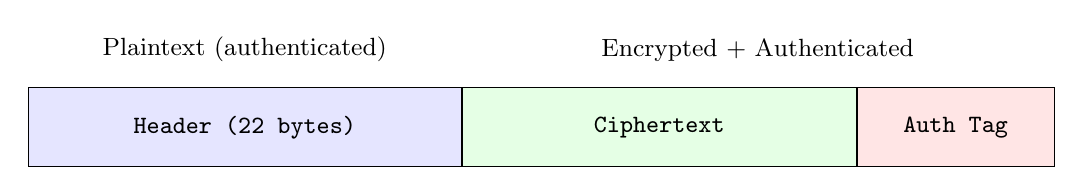
\begin{tikzpicture}[
  field/.style={draw, minimum height=1cm, font=\ttfamily\small},
]
  \node[field, minimum width=5.5cm, fill=blue!10] (hdr) at (0,0) {Header (22 bytes)};
  \node[field, minimum width=5cm, fill=green!10, anchor=west] (ct) at (hdr.east) {Ciphertext};
  \node[field, minimum width=2.5cm, fill=red!10, anchor=west] (tag) at (ct.east) {Auth Tag};

  \node[above=0.2cm, font=\small] at (hdr.north) {Plaintext (authenticated)};
  \node[above=0.2cm, font=\small] at ([xshift=1.25cm]ct.north) {Encrypted + Authenticated};
\end{tikzpicture}
\end{center}

The header is transmitted in plaintext but is included as
\emph{associated data} in the AEAD computation, so any tampering
with header fields causes authentication failure at the receiver.

The initialisation vector (IV/nonce) is \emph{not} transmitted on
the wire.  Instead, it is reconstructed by the receiver from the
\texttt{epoch} and \texttt{seq} fields in the header, saving 12~bytes
per packet.

% ============================================================
\section{Header Format}
\label{sec:wire-header}

The header is packed using Python's \texttt{struct} module with the
format string:

\begin{lstlisting}[style=python]
HEADER_STRUCT = "!BBBBB8sQB"
# Total: 1+1+1+1+1+8+8+1 = 22 bytes
\end{lstlisting}

The \texttt{!} prefix specifies network byte order (big-endian).
Each field is detailed in Table~\ref{tab:header-fields}.

\begin{table}[htbp]
\centering
\caption{AEAD header fields (22 bytes total).}
\label{tab:header-fields}
\begin{tabular}{c l c l p{4.5cm}}
  \toprule
  \textbf{Offset} & \textbf{Field} & \textbf{Size} & \textbf{Format} & \textbf{Description} \\
  \midrule
  0  & \texttt{version}    & 1\,B  & \texttt{B} (uint8) & Wire protocol version; always 1 \\
  1  & \texttt{kem\_id}    & 1\,B  & \texttt{B} (uint8) & KEM algorithm family identifier \\
  2  & \texttt{kem\_param} & 1\,B  & \texttt{B} (uint8) & KEM parameter set within family \\
  3  & \texttt{sig\_id}    & 1\,B  & \texttt{B} (uint8) & Signature algorithm family ID \\
  4  & \texttt{sig\_param} & 1\,B  & \texttt{B} (uint8) & Signature parameter set within family \\
  5  & \texttt{session\_id}& 8\,B  & \texttt{8s} (bytes) & Random session identifier \\
  13 & \texttt{seq}        & 8\,B  & \texttt{Q} (uint64) & Packet sequence number \\
  21 & \texttt{epoch}      & 1\,B  & \texttt{B} (uint8) & Key epoch (0--255) \\
  \bottomrule
\end{tabular}
\end{table}

\subsection{Field Semantics}

\paragraph{version.}
Fixed at~1 for the current protocol.  The receiver rejects any packet
whose version does not match.  This field enables future protocol
evolution without ambiguity.

\paragraph{kem\_id and kem\_param.}
Together these two bytes identify the KEM algorithm.  For example,
ML-KEM-768 might map to \texttt{kem\_id=1, kem\_param=2}.  The
mapping is defined in the \classname{AeadIds} named tuple and the
suite registry (Chapter~\ref{ch:suites}).

\paragraph{sig\_id and sig\_param.}
Analogous to the KEM identifiers but for the signature algorithm
used during the handshake.  These allow the receiver to verify that
the packet comes from a session established with the expected
cryptographic parameters.

\paragraph{session\_id.}
Eight bytes of random data generated during the handshake.  Both
sides derive the same session ID from the shared secret using HKDF.
The receiver checks that the session ID matches; mismatches indicate
either a stale packet from a previous session or a spoofing attempt.

\paragraph{seq.}
A 64-bit unsigned integer that starts at~0 and increments by~1 for
each packet sent.  This field serves two purposes:
\begin{enumerate}
  \item \textbf{Nonce construction}: Combined with \texttt{epoch}, it
        provides a unique IV for every AEAD operation.
  \item \textbf{Anti-replay}: The receiver maintains a sliding window
        and rejects packets with sequence numbers that fall outside
        the window or have already been seen.
\end{enumerate}

\paragraph{epoch.}
A single byte (0--255) that increments when the sender calls
\funcname{bump\_epoch}.  Each epoch reset sets \texttt{seq} back
to~0.  The combination of \texttt{epoch} and \texttt{seq} ensures
nonce uniqueness even across epoch boundaries.  Wrapping from
255 to~0 is \emph{forbidden} with the same key material; a new
handshake must be performed.

% ============================================================
\section{Nonce Construction}
\label{sec:wire-nonce}

The AEAD nonce is reconstructed at both sender and receiver using
the \funcname{\_build\_nonce} function.  For AES-GCM and
ChaCha20-Poly1305 the nonce is 12~bytes:

\begin{center}
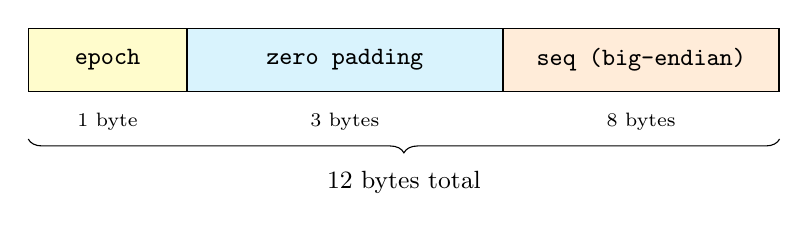
\begin{tikzpicture}[
  field/.style={draw, minimum height=0.8cm, font=\ttfamily\small},
]
  \node[field, minimum width=2cm, fill=yellow!20] (epoch) at (0,0) {epoch};
  \node[field, minimum width=4cm, fill=cyan!15, anchor=west] (pad) at (epoch.east) {zero padding};
  \node[field, minimum width=3.5cm, fill=orange!15, anchor=west] (seq) at (pad.east) {seq (big-endian)};
  
  \node[below=0.15cm, font=\scriptsize] at (epoch.south) {1 byte};
  \node[below=0.15cm, font=\scriptsize] at (pad.south) {3 bytes};
  \node[below=0.15cm, font=\scriptsize] at (seq.south) {8 bytes};
  
  \draw[decorate, decoration={brace, mirror, amplitude=5pt}]
    ([yshift=-0.6cm]epoch.south west) -- ([yshift=-0.6cm]seq.south east)
    node[midway, below=8pt, font=\small] {12 bytes total};
\end{tikzpicture}
\end{center}

The construction is:
\begin{lstlisting}[style=python]
def _build_nonce(epoch: int, seq: int, nonce_len: int) -> bytes:
    epoch_bytes = epoch.to_bytes(1, "big")
    seq_bytes   = seq.to_bytes(8, "big")
    padding     = b"\x00" * (nonce_len - 1 - 8)
    return epoch_bytes + padding + seq_bytes
\end{lstlisting}

For ASCON-128a, the nonce is 16~bytes (7~bytes of padding instead
of~3).

\begin{keyinsight}{Why not transmit the nonce?}
  Classical TLS and DTLS transmit the nonce (or a portion of it) in
  every record.  By deriving the nonce from header fields that are
  already transmitted (\texttt{epoch} and \texttt{seq}), the system
  saves 12~bytes per packet.  On a MAVLink stream at 50~packets/second,
  this is \SI{600}{B/s}---small but meaningful on bandwidth-constrained
  radio links.
\end{keyinsight}

% ============================================================
\section{Complete Packet Layout}

Combining all components, a full encrypted packet looks like this:

\begin{center}
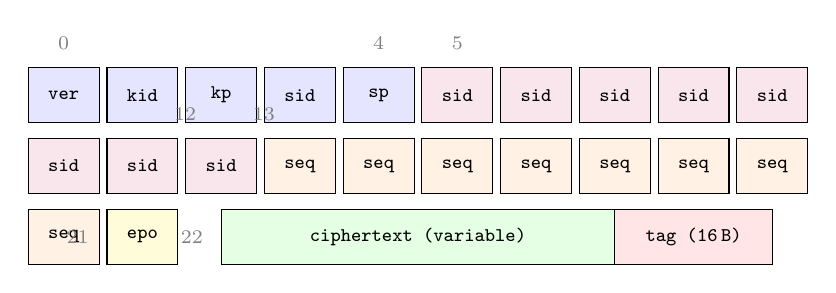
\begin{tikzpicture}[
  byte/.style={draw, minimum height=0.7cm, minimum width=0.9cm, font=\scriptsize\ttfamily},
  label/.style={font=\scriptsize, text=gray},
]
  % Row 1: bytes 0-9
  \foreach \i/\lbl in {0/ver, 1/kid, 2/kp, 3/sid, 4/sp} {
    \node[byte, fill=blue!10] (b\i) at (\i*1, 0) {\lbl};
  }
  \foreach \i in {5,6,7,8,9} {
    \node[byte, fill=purple!10] (b\i) at (\i*1, 0) {sid};
  }
  % Row 2: bytes 10-19
  \foreach \i in {10,11,12} {
    \node[byte, fill=purple!10] (b\i) at ({(\i-10)*1}, -0.9) {sid};
  }
  \foreach \i in {13,14,15,16,17,18,19} {
    \node[byte, fill=orange!10] (b\i) at ({(\i-10)*1}, -0.9) {seq};
  }
  % Row 3: bytes 20-21 + ciphertext
  \node[byte, fill=orange!10] (b20) at (0, -1.8) {seq};
  \node[byte, fill=yellow!15] (b21) at (1, -1.8) {epo};
  \node[byte, fill=green!10, minimum width=5cm] (ct) at (4.5, -1.8) {ciphertext (variable)};
  \node[byte, fill=red!10, minimum width=2cm] (tag) at (8, -1.8) {tag (16\,B)};
  
  % Labels
  \node[label, above=0.1cm] at (b0.north) {0};
  \node[label, above=0.1cm] at (b4.north) {4};
  \node[label, above=0.1cm] at (b5.north) {5};
  \node[label, above=0.1cm] at (b12.north west) {12};
  \node[label, above=0.1cm] at (b13.north west) {13};
  \node[label, left=0.1cm] at (b21.west) {21};
  \node[label, left=0.1cm] at (ct.west) {22};
\end{tikzpicture}
\end{center}

\noindent
\textbf{Legend:}
\texttt{ver} = version,
\texttt{kid} = kem\_id,
\texttt{kp} = kem\_param,
\texttt{sid} = sig\_id (byte 3) / session\_id (bytes 5--12),
\texttt{sp} = sig\_param,
\texttt{seq} = sequence number (bytes 13--20),
\texttt{epo} = epoch.

% ============================================================
\section{Packet Size Analysis}

For a typical MAVLink v2 packet of $P$~payload bytes, the total
encrypted packet size is:

\[
  \text{Total} = \underbrace{22}_{\text{header}}
               + \underbrace{P}_{\text{ciphertext}}
               + \underbrace{16}_{\text{auth tag}}
  = P + 38 \text{ bytes}
\]

\begin{table}[htbp]
\centering
\caption{Packet sizes for representative MAVLink messages.}
\label{tab:packet-sizes}
\begin{tabular}{l c c c}
  \toprule
  \textbf{MAVLink Message} & \textbf{Payload} & \textbf{Encrypted} & \textbf{Overhead} \\
  \midrule
  HEARTBEAT              &  9\,B  &  47\,B & 422\% \\
  ATTITUDE               & 28\,B  &  66\,B &  136\% \\
  GPS\_RAW\_INT           & 30\,B  &  68\,B &  127\% \\
  GLOBAL\_POSITION\_INT   & 28\,B  &  66\,B &  136\% \\
  MISSION\_ITEM\_INT      & 37\,B  &  75\,B &  103\% \\
  Typical (avg.\ $\sim$50) & 50\,B  &  88\,B &   76\% \\
  MTU-filling             & 1200\,B & 1238\,B &  3.2\% \\
  \bottomrule
\end{tabular}
\end{table}

The overhead is substantial for small heartbeat packets but drops
to single-digit percentages for larger payloads.  In practice,
MAVLink heartbeats are sent at \SI{1}{\hertz}, so the absolute
bandwidth cost of the overhead is only $\sim$38~bytes/second.

% ============================================================
\section{Authentication Tag}

The authentication tag is produced by the AEAD algorithm:

\begin{itemize}
  \item \textbf{AES-256-GCM}: 16~bytes (128-bit tag)
  \item \textbf{ChaCha20-Poly1305}: 16~bytes (128-bit tag)
  \item \textbf{ASCON-128a}: 16~bytes (128-bit tag)
\end{itemize}

All three algorithms produce the same tag length, keeping the wire
format consistent regardless of AEAD choice.

% ============================================================
\section{Replay Protection on the Wire}

The receiver maintains a sliding window of size
$W = \configkey{REPLAY\_WINDOW}$ (default 1024).  For each
incoming packet with sequence number $s$:

\begin{enumerate}
  \item If $s > s_{\max}$: accept (new high-water mark); advance
        window.
  \item If $s_{\max} - W < s \le s_{\max}$: check bitmap; accept
        if not yet seen, reject if duplicate.
  \item If $s \le s_{\max} - W$: reject (too old).
\end{enumerate}

A packet is only marked as ``seen'' in the bitmap \emph{after}
successful AEAD authentication.  This prevents an attacker from
burning sequence numbers by sending forged packets.

% ============================================================
\section{Session ID Derivation}

The 8-byte session ID is derived during the handshake using HKDF:

\begin{lstlisting}[style=python]
session_id = HKDF(
    algorithm = SHA-256,
    length    = 8,
    salt      = None,
    info      = b"pqc-session-id",
    ikm       = shared_secret
)
\end{lstlisting}

Both sides derive the same session ID from the same shared secret,
providing a cryptographic binding between the handshake and the
data plane.
